\documentclass[12pt,oneside]{book}

%\usepackage{subfiles}
\usepackage{tikz}
\usetikzlibrary{arrows,automata}
\usepackage[notextcomp]{kpfonts} 
%\usepackage{kmath,kerkis}
\usepackage{graphicx}
\usepackage{eurosym}
\usepackage{amsfonts}
\usepackage{amsmath}
\usepackage{amssymb}
\usepackage{stmaryrd}
\usepackage{amsthm}
\usepackage[margin=1in]{geometry}
\usepackage[hang,flushmargin,symbol*]{footmisc}
\usepackage{color}
\definecolor{darkblue}{rgb}{0, 0, .6}
\definecolor{grey}{rgb}{.7, .7, .7}
\usepackage[breaklinks]{hyperref}
\hypersetup{
	colorlinks=true,
	linkcolor=darkblue,
	anchorcolor=darkblue,
	citecolor=darkblue,
	pagecolor=darkblue,
	urlcolor=darkblue,
	pdftitle={},
	pdfauthor={}
}

\usepackage{fancyhdr}
\pagestyle{fancy}
\lhead{\leftmark}
\chead{}
\rhead{}
\lfoot{}
\cfoot{}
\rfoot{}

\theoremstyle{definition}
\newtheorem{theorem}{Theorem}[chapter]
\newtheorem{acknowledgement}[theorem]{Acknowledgement}
\newtheorem{algorithm}[theorem]{Algorithm}
\newtheorem{axiom}[theorem]{Axiom}
\newtheorem{case}[theorem]{Case}
\newtheorem{claim}[theorem]{Claim}
\newtheorem{conclusion}[theorem]{Conclusion}
\newtheorem{condition}[theorem]{Condition}
\newtheorem{conjecture}[theorem]{Conjecture}
\newtheorem{corollary}[theorem]{Corollary}
\newtheorem{criterion}[theorem]{Criterion}
\newtheorem{definition}[theorem]{Definition}
\newtheorem{example}[theorem]{Example}
\newtheorem{exercise}[theorem]{Exercise}
\newtheorem{journal}[theorem]{Journal}
\newtheorem{lemma}[theorem]{Lemma}
\newtheorem{notation}[theorem]{Notation}
\newtheorem{problem}[theorem]{Problem}
\newtheorem{proposition}[theorem]{Proposition}
\newtheorem{remark}[theorem]{Remark}
\newtheorem{solution}[theorem]{Solution}
\newtheorem{summary}[theorem]{Summary}
\newtheorem{skeleton}[theorem]{Skeleton Proof}
\newtheorem{activity}[theorem]{Activity}

\newsavebox{\savepar}
\newenvironment{textbox}{\noindent\begin{lrbox}{\savepar}\begin{minipage}[c]{.98\textwidth}}{\end{minipage}\end{lrbox}\fcolorbox{black}{white}{\usebox{\savepar}}}

\newcommand{\dom}{\operatorname{Dom}}
\newcommand{\codom}{\operatorname{Codom}}
\newcommand{\range}{\operatorname{Rng}}

\begin{document}

\title{An Inquiry-Based Approach to Abstract Algebra}
\author{Dana C.~Ernst, PhD\\
Northern Arizona University}
\date{Fall 2013}

\maketitle
\thispagestyle{empty}

\noindent\copyright{ \the\year\ Dana C.~Ernst.  Some Rights Reserved.\\

\bigskip

\noindent This work is licensed under the Creative Commons Attribution-Share Alike 3.0 United States License.  You may copy, distribute, display, and perform this copyrighted work, but only if you give credit to Dana C.~Ernst, and all derivative works based upon it must be published under the Creative Commons Attribution-Share Alike 3.0 United States License. Please attribute this work to Dana C.~Ernst, Mathematics Faculty at Northern Arizona University, \url{dana.ernst@nau.edu}. To view a copy of this license, visit
\begin{center}
\url{http://creativecommons.org/licenses/by-sa/3.0/us/}
\end{center}
or send a letter to Creative Commons, 171 Second Street, Suite 300, San Francisco, California, 94105, USA.}

\bigskip

\begin{center}

\includegraphics{by-sa.png}
\end{center}

\noindent Here is a partial list of people that I need to thank for supplying content, advice, and feedback.
\begin{itemize}
\item Ben Woodruff
\item Josh Wiscons
\item Dave Richeson
\item Nathan Carter
\item \emph{The Elements of Style for Proofs} (see Appendix~\ref{appendix:elements_of_style}) is a blending of work by \href{http://www.cord.edu/faculty/ahendric/}{Anders Hendrickson} and Dave Richeson.
\end{itemize}

\tableofcontents
\thispagestyle{empty}

%\chapter*{Acknowledgements}
\addcontentsline{toc}{chapter}{\protect\numberline{}Acknowledgements}

\noindent This book has been an open-source project since day one. Instructors and students can download the PDF for free and modify the source as they see fit. Several of instructors and students have provided extremely useful feedback, which has improved the book at each iteration. Moreover, due to the open-source nature of the book, I have been able to incorporate content written by others. Below is a list of people (alphabetical by last name) that have contributed content, advice, or feedback.

\begin{itemize}
\item \href{https://faculty.bentley.edu/details.asp?uname=ncarter}{Nathan Carter} (Bentley University). Nathan's excellent book \emph{Visual Group Theory} has had a huge impact on my approach to teaching abstract algebra.
\item \href{https://www.linkedin.com/in/andershendrickson/}{Anders Hendrickson} (Milliman). Anders is the original author of the content in Appendix~\ref{appendix:elements_of_style}: Elements of Style for Proofs. The current version in Appendix~\ref{appendix:elements_of_style} is a result of modifications made by myself with some suggestions from David Richeson.
%\item \href{https://embracinglifewithmajorrevisions.org/2017/07/12/rights-of-the-learner-an-introduction/}{Crystal Kalinec-Craig} (University of Texas at San Antonio). Section~\ref{sec:Rights of the Learner}: Rights of the Learner is an adaptation of a similar list written by Crystal.
\item \href{http://www.math.clemson.edu/~macaule/}{Matthew Macauley} (Clemson University).  Several Cayley diagrams throughout the book were borrowed from or inspired by Matt.
\item \href{https://ericwmiles.weebly.com}{Eric Miles} (Colorado Mesa University). Eric modified an earlier version of the book. I reincorporated several of his improvements.
\item \href{http://users.dickinson.edu/~richesod/}{David Richeson} (Dickinson College). David is responsible for much of the content in Appendix~\ref{appendix:fancy_math_terms}: Fancy Mathematical Terms and Appendix~\ref{appendix:definitions}: Definitions in Mathematics.
\item \href{http://webpages.csus.edu/wiscons/}{Josh Wiscons} (CSU Sacramento) and \href{http://emp.byui.edu/woodruffb/}{Ben Woodruff} (BYU Idaho). In the early stages of development, Josh and Ben were instrumental in the development of this book.
\end{itemize}

\chapter{Introduction}

\begin{section}{What is Abstract Algebra?}

Abstract algebra is the subject area of mathematics that studies algebraic structures, such as groups, rings, fields, modules, vector spaces, and algebras. This course is an introduction to abstract algebra. We will spend most of our time studying groups. Group theory is the study of symmetry, and is one of the most beautiful areas in all of mathematics. It arises in puzzles, visual arts, music, nature, the physical and life sciences, computer science, cryptography, and of course, throughout mathematics. This course will cover the basic concepts of group theory, and a special effort will be made to emphasize the intuition behind the concepts and motivate the subject matter.  In the last few weeks of the semester, we will also introduce rings and fields.
\epigraph{The mathematician does not study pure mathematics because it is useful; he studies it because he delights in it, and he delights in it because it is beautiful.}{\emph{Henri Poincar\'e}}

\end{section}

\begin{section}{An Inquiry-Based Approach}

This is not a lecture-oriented class or one in which mimicking prefabricated examples will lead you to success. You will be expected to work actively to construct your own understanding of the topics at hand with the readily available help of me and your classmates. Many of the concepts you learn and problems you work on will be new to you and ask you to stretch your thinking. You will experience \emph{frustration} and \emph{failure} before you experience \emph{understanding}. This is part of the normal learning process. If you are doing things well, you should be confused at different points in the semester. The material is too rich for a human being to completely understand it immediately. Your viability as a professional in the modern workforce depends on your ability to embrace this learning process and make it work for you.

\epigraph{Don't fear failure.  Not failure, but low aim, is the crime. In great attempts it is glorious even to fail.}{\emph{Bruce Lee}}

In order to promote a more active participation in your learning, we will incorporate ideas from an educational philosophy called inquiry-based learning (IBL).  Loosely speaking, IBL is a student-centered method of teaching mathematics that engages students in sense-making activities.  Students are given tasks requiring them to solve problems, conjecture, experiment, explore, create, and communicate.  Rather than showing facts or a clear, smooth path to a solution, the instructor guides and mentors students via well-crafted problems through an adventure in mathematical discovery.  According to \href{https://www.colorado.edu/eer/sites/default/files/attached-files/laursenrasmussencommentaryauthorversion0219.pdf}{Laursen and Rasmussen (2019)}, the Four Pillars of IBL are:
\begin{itemize}
\item Students engage deeply with coherent and meaningful mathematical tasks.
\item Students collaboratively process mathematical ideas.
\item Instructors inquire into student thinking.
\item Instructors foster equity in their design and facilitation choices.
\end{itemize}

Much of the course will be devoted to students presenting their proposed solutions or proofs on the board and a significant portion of your grade will be determined by how much mathematics you produce.  I use the word \emph{produce} because I believe that the best way to learn mathematics is by doing mathematics.  Someone cannot master a musical instrument or a martial art by simply watching, and in a similar fashion, you cannot master mathematics by simply watching; you must do mathematics!

In any act of creation, there must be room for experimentation, and thus allowance for mistakes, even failure. A key goal of our community is that we support each other---sharpening each other's thinking but also bolstering each other's confidence---so that we can make failure a productive experience. Mistakes are inevitable, and they should not be an obstacle to further progress. It's normal to struggle and be confused as you work through new material. Accepting that means you can keep working even while feeling stuck, until you overcome and reach even greater accomplishments.

\epigraph{You will become clever through your mistakes.}{\emph{German Proverb}}

Furthermore, it is important to understand that solving genuine problems is difficult and takes time.  You shouldn't expect to complete each problem in 10 minutes or less.  Sometimes, you might have to stare at the problem for an hour before even understanding how to get started.

In this course, everyone will be required to
\begin{itemize}
\item read and interact with course notes and textbook on your own;
\item write up quality solutions/proofs to assigned problems;
\item present solutions/proofs on the board to the rest of the class;
\item participate in discussions centered around a student's presented solution/proof;
\item call upon your own prodigious mental faculties to respond in flexible, thoughtful, and creative ways to problems that may seem unfamiliar on first glance.
\end{itemize}
As the semester progresses, it should become clear to you what the expectations are.

\epigraph{Tell me and I forget, teach me and I may remember, involve me and I learn.}{\emph{Benjamin Franklin}}

\end{section}

\begin{section}{Rights of the Learner}
As a student in this class, you have the right:
\begin{enumerate}
\item to be confused,
\item to make a mistake and to revise your thinking,
\item to speak, listen, and be heard, and
\item to enjoy doing mathematics.
\end{enumerate}

\epigraph{You may encounter many defeats, but you must not be defeated.}{\emph{Maya Angelou}}
	
\end{section}

\begin{section}{Structure of the Notes}

As you read the notes, you will be required to digest the material in a meaningful way.  It is your responsibility to read and understand new definitions and their related concepts.  However, you will be supported in this sometimes difficult endeavor. In addition, you will be asked to complete problems aimed at solidifying your understanding of the material.  Most importantly, you will be asked to make conjectures, produce counterexamples, and prove theorems.

The items labeled as \textbf{Definition} and \textbf{Example} are meant to be read and digested.  However, the items labeled as \textbf{Problem}, \textbf{Theorem}, and \textbf{Corollary} require action on your part.  Items labeled as \textbf{Problem} are sort of a mixed bag. Some Problems are computational in nature and aimed at improving your understanding of a particular concept while others ask you to provide a counterexample for a statement if it is false or to provide a proof if the statement is true. Items with the \textbf{Theorem} and \textbf{Corollary} designation are mathematical facts and the intention is for you to produce a valid proof of the given statement.  The main difference between a \textbf{Theorem} and a \textbf{Corollary} is that corollaries are typically statements that follow quickly from a previous theorem.  In general, you should expect corollaries to have very short proofs.  However, that doesn't mean that you can't produce a more lengthy yet valid proof of a corollary.

It is important to point out that there are very few examples in the notes.  This is intentional.  One of the goals of the items labeled as \textbf{Problem} is for you to produce the examples.

Lastly, there are many situations where you will want to refer to an earlier definition, problem, theorem, or corollary.  In this case, you should reference the statement by number.  For example, you might write something like, ``By Theorem~\ref{thm:order_element_divides_group_order}, we see that\ldots."

\end{section}

\begin{section}{Some Minimal Guidance}
Especially in the opening sections, it won't be clear what facts from your prior experience in mathematics we are ``allowed" to use.  Unfortunately, addressing this issue is difficult and is something we will sort out along the way.  However, in general, here are some minimal guidelines to keep in mind.  

First, there are times when we will need to do some basic algebraic manipulations.  You should feel free to do this whenever the need arises.  But you should show sufficient work along the way.  You do not need to write down justifications for basic algebraic manipulations (e.g., adding 1 to both sides of an equation, adding and subtracting the same amount on the same side of an equation, adding like terms, factoring, basic simplification, etc.).  

On the other hand, you do need to make explicit justification of the logical steps in a proof.  When necessary, you should cite a previous definition, theorem, etc. by number.

Unlike the experience many of you had writing proofs in geometry, our proofs will be written in complete sentences.  You should break sections of a proof into paragraphs and use proper grammar.  There are some pedantic conventions for doing this that I will point out along the way.  Initially, this will be an issue that most students will struggle with, but after a few weeks everyone will get the hang of it.

Ideally, you should rewrite the statements of theorems before you start the proof.  Moreover, for your sake and mine, you should label the statement with the appropriate number.  I will expect you to indicate where the proof begins by writing ``\emph{Proof.}" at the beginning.  Also, we will conclude our proofs with the standard ``proof box" (i.e., $\square$ or $\blacksquare$), which is typically right-justified.

Lastly, every time you write a proof, you need to make sure that you are making your assumptions crystal clear.  Sometimes there will be some implicit assumptions that we can omit, but at least in the beginning, you should get in the habit of stating your assumptions up front.  Typically, these statements will start off ``Assume\ldots" or ``Let\ldots".  

This should get you started.  We will discuss more as the semester progresses.  Now, go have fun and kick some butt!

\epigraph{If you want to sharpen a sword, you have to remove a little metal.}{\emph{Unknown}}

\end{section}
\chapter{Prerequisites}
\label{chapter:prerequisites}

blah
\chapter{An Intuitive Approach to Groups}
\label{chapter:intuitive_approach_groups}
\thispagestyle{empty}

One of the major topics of this course is \textbf{groups}.  The area of mathematics that is concerned with groups is called \textbf{group theory}. Loosely speaking, group theory is the study of symmetry, and in my opinion is one of the most beautiful areas in all of mathematics. It arises in puzzles, visual arts, music, nature, the physical and life sciences, computer science, cryptography, and of course, throughout mathematics.

Instead of starting with an abstract formal definition, we will begin our study of groups by developing some intuition about what groups actually are.  To get started, we will be exploring the game Spinpossible\texttrademark, which is a free game that is available for iOS and Android devices. Alternatively, you can just play the game in any modern web browser (\url{https://spinpossible.com}).  The game is played on a $3\times 3$ board of scrambled tiles numbered 1 to 9, each of which may be right-side-up or up-side-down. The objective of the game is to return the board to the standard configuration where tiles are arranged in numerical order and right-side-up. This is accomplished by a sequence of ``spins", where a spin consists of rotating an $m\times n$ subrectangle by 180$^\circ$. The goal is to minimize the number of spins used.  The following figure depicts a scrambled board on the left and the solved board on the right.  The sequence of arrows is used to denote some sequence of spins that transforms the scrambled board into the solved board.

\begin{center}
\begin{tabular}{c}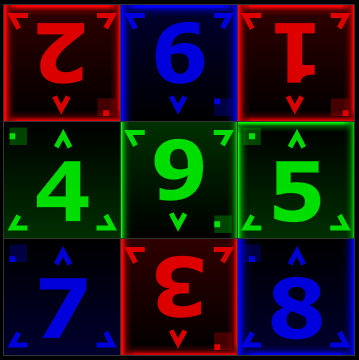
\includegraphics[width=1.5in]{scramble1.PNG}\end{tabular}
{\large $\xrightarrow{?} \cdots \xrightarrow{?}$}
\begin{tabular}{c}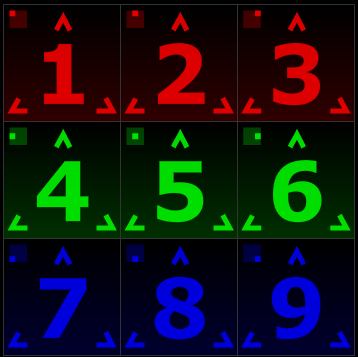
\includegraphics[width=1.5in]{scramble4.PNG}\end{tabular}
\end{center}

\begin{example}\label{ex:spinpossible}
Let's play with an example.  Suppose we start with the following scrambled board.

\begin{center}
\begin{tikzpicture}[every node/.style={minimum size=.65cm}]
  \node [draw] (1) {\rotatebox{180}{$\underline{2}$}};
  \node [draw, right=0cm of 1] (2) {\rotatebox{180}{$\underline{9}$}};
  \node [draw, right=0cm of 2] (3) {\rotatebox{180}{$\underline{1}$}};
  \node [draw, below=0cm of 1] (4) {$\underline{4}$};
  \node [draw, right=0cm of 4] (5) {\rotatebox{180}{$\underline{6}$}};
  \node [draw, right=0cm of 5] (6) {$\underline{5}$};
  \node [draw, below=0cm of 4] (7) {$\underline{7}$};
  \node [draw, right=0cm of 7] (8) {\rotatebox{180}{$\underline{3}$}};
  \node [draw, right=0cm of 8] (9) {$\underline{8}$};
\end{tikzpicture}
\end{center}

\noindent The underlines on the numbers are meant to help us tell whether a tile is right-side-up or up-side-down.  Our goal is to use a sequence of spins to unscramble the board.  Before we get started, let's agree on some conventions.  When we refer to tile $n$, we mean the actual tile that is labeled by the number $n$ regardless of its position and orientation on the board.  On the other hand, position $n$ will refer to the position on the board that tile $n$ is supposed to be in when the board has been unscrambled.  For example, in the board above, tile 1 is in position 3 and tile 7 happens to be in position 7.  

It turns out that there are multiple ways to unscramble this board., but I have one particular sequence in mind.  First, let's spin the rectangle determined by the two rightmost columns.  Here's what we get.  I've shaded the subrectangle that we are spinning.

\begin{center}
\begin{tabular}{c}
\begin{tikzpicture}[every node/.style={minimum size=.65cm}]
  \node [draw] (1) {\rotatebox{180}{$\underline{2}$}};
  \node [draw, fill=blue!40, right=0cm of 1] (2) {\rotatebox{180}{$\underline{9}$}};
  \node [draw, fill=blue!40, right=0cm of 2] (3) {\rotatebox{180}{$\underline{1}$}};
  \node [draw, below=0cm of 1] (4) {$\underline{4}$};
  \node [draw, fill=blue!40, right=0cm of 4] (5) {\rotatebox{180}{$\underline{6}$}};
  \node [draw, fill=blue!40, right=0cm of 5] (6) {$\underline{5}$};
  \node [draw, below=0cm of 4] (7) {$\underline{7}$};
  \node [draw, fill=blue!40, right=0cm of 7] (8) {\rotatebox{180}{$\underline{3}$}};
  \node [draw, fill=blue!40, right=0cm of 8] (9) {$\underline{8}$};
\end{tikzpicture}
\end{tabular}
%
{\large $\rightarrow$}
%
\begin{tabular}{c}
\begin{tikzpicture}[every node/.style={minimum size=.65cm}]
  \node [draw] (1) {\rotatebox{180}{$\underline{2}$}};
  \node [draw, right=0cm of 1] (2) {\rotatebox{180}{$\underline{8}$}};
  \node [draw, right=0cm of 2] (3) {$\underline{3}$};
  \node [draw, below=0cm of 1] (4) {$\underline{4}$};
  \node [draw, right=0cm of 4] (5) {\rotatebox{180}{$\underline{5}$}};
  \node [draw, right=0cm of 5] (6) {$\underline{6}$};
  \node [draw, below=0cm of 4] (7) {$\underline{7}$};
  \node [draw, right=0cm of 7] (8) {$\underline{1}$};
  \node [draw, right=0cm of 8] (9) {$\underline{9}$};
\end{tikzpicture}
\end{tabular}
\end{center}

\noindent Okay, now let's spin the middle column.

\begin{center}
\begin{tabular}{c}
\begin{tikzpicture}[every node/.style={minimum size=.65cm}]
  \node [draw] (1) {\rotatebox{180}{$\underline{2}$}};
  \node [draw, fill=blue!40, right=0cm of 1] (2) {\rotatebox{180}{$\underline{8}$}};
  \node [draw, right=0cm of 2] (3) {$\underline{3}$};
  \node [draw, below=0cm of 1] (4) {$\underline{4}$};
  \node [draw, fill=blue!40, right=0cm of 4] (5) {\rotatebox{180}{$\underline{5}$}};
  \node [draw, right=0cm of 5] (6) {$\underline{6}$};
  \node [draw, below=0cm of 4] (7) {$\underline{7}$};
  \node [draw, fill=blue!40, right=0cm of 7] (8) {$\underline{1}$};
  \node [draw, right=0cm of 8] (9) {$\underline{9}$};
\end{tikzpicture}
\end{tabular}
%
{\large $\rightarrow$}
%
\begin{tabular}{c}
\begin{tikzpicture}[every node/.style={minimum size=.65cm}]
  \node [draw] (1) {\rotatebox{180}{$\underline{2}$}};
  \node [draw, right=0cm of 1] (2) {\rotatebox{180}{$\underline{1}$}};
  \node [draw, right=0cm of 2] (3) {$\underline{3}$};
  \node [draw, below=0cm of 1] (4) {$\underline{4}$};
  \node [draw, right=0cm of 4] (5) {$\underline{5}$};
  \node [draw, right=0cm of 5] (6) {$\underline{6}$};
  \node [draw, below=0cm of 4] (7) {$\underline{7}$};
  \node [draw, right=0cm of 7] (8) {$\underline{8}$};
  \node [draw, right=0cm of 8] (9) {$\underline{9}$};
\end{tikzpicture}
\end{tabular}
\end{center}

\noindent Hopefully, you can see that we are really close to unscrambling the board.  All we need to do is spin the rectangle determined by the tiles in positions 1 and 2.

\begin{center}
\begin{tabular}{c}
\begin{tikzpicture}[every node/.style={minimum size=.65cm}]
  \node [draw, fill=blue!40] (1) {\rotatebox{180}{$\underline{2}$}};
  \node [draw, fill=blue!40, right=0cm of 1] (2) {\rotatebox{180}{$\underline{1}$}};
  \node [draw, right=0cm of 2] (3) {$\underline{3}$};
  \node [draw, below=0cm of 1] (4) {$\underline{4}$};
  \node [draw, right=0cm of 4] (5) {$\underline{5}$};
  \node [draw, right=0cm of 5] (6) {$\underline{6}$};
  \node [draw, below=0cm of 4] (7) {$\underline{7}$};
  \node [draw, right=0cm of 7] (8) {$\underline{8}$};
  \node [draw, right=0cm of 8] (9) {$\underline{9}$};
\end{tikzpicture}
\end{tabular}
%
{\large $\rightarrow$}
%
\begin{tabular}{c}
\begin{tikzpicture}[every node/.style={minimum size=.65cm}]
  \node [draw] (1) {$\underline{1}$};
  \node [draw, right=0cm of 1] (2) {$\underline{2}$};
  \node [draw, right=0cm of 2] (3) {$\underline{3}$};
  \node [draw, below=0cm of 1] (4) {$\underline{4}$};
  \node [draw, right=0cm of 4] (5) {$\underline{5}$};
  \node [draw, right=0cm of 5] (6) {$\underline{6}$};
  \node [draw, below=0cm of 4] (7) {$\underline{7}$};
  \node [draw, right=0cm of 7] (8) {$\underline{8}$};
  \node [draw, right=0cm of 8] (9) {$\underline{9}$};
\end{tikzpicture}
\end{tabular}
\end{center}

\noindent Putting all of our moves together, here is what we have.

\begin{center}
\begin{tabular}{c}
\begin{tikzpicture}[every node/.style={minimum size=.65cm}]
  \node [draw] (1) {\rotatebox{180}{$\underline{2}$}};
  \node [draw, fill=blue!40, right=0cm of 1] (2) {\rotatebox{180}{$\underline{9}$}};
  \node [draw, fill=blue!40, right=0cm of 2] (3) {\rotatebox{180}{$\underline{1}$}};
  \node [draw, below=0cm of 1] (4) {$\underline{4}$};
  \node [draw, fill=blue!40, right=0cm of 4] (5) {\rotatebox{180}{$\underline{6}$}};
  \node [draw, fill=blue!40, right=0cm of 5] (6) {$\underline{5}$};
  \node [draw, below=0cm of 4] (7) {$\underline{7}$};
  \node [draw, fill=blue!40, right=0cm of 7] (8) {\rotatebox{180}{$\underline{3}$}};
  \node [draw, fill=blue!40, right=0cm of 8] (9) {$\underline{8}$};
\end{tikzpicture}
\end{tabular}
%
{\large $\rightarrow$}
%
\begin{tabular}{c}
\begin{tikzpicture}[every node/.style={minimum size=.65cm}]
  \node [draw] (1) {\rotatebox{180}{$\underline{2}$}};
  \node [draw, fill=blue!40, right=0cm of 1] (2) {\rotatebox{180}{$\underline{8}$}};
  \node [draw, right=0cm of 2] (3) {$\underline{3}$};
  \node [draw, below=0cm of 1] (4) {$\underline{4}$};
  \node [draw, fill=blue!40, right=0cm of 4] (5) {\rotatebox{180}{$\underline{5}$}};
  \node [draw, right=0cm of 5] (6) {$\underline{6}$};
  \node [draw, below=0cm of 4] (7) {$\underline{7}$};
  \node [draw, fill=blue!40, right=0cm of 7] (8) {$\underline{1}$};
  \node [draw, right=0cm of 8] (9) {$\underline{9}$};
\end{tikzpicture}
\end{tabular}
%
{\large $\rightarrow$}
%
\begin{tabular}{c}
\begin{tikzpicture}[every node/.style={minimum size=.65cm}]
  \node [draw, fill=blue!40] (1) {\rotatebox{180}{$\underline{2}$}};
  \node [draw, fill=blue!40, right=0cm of 1] (2) {\rotatebox{180}{$\underline{1}$}};
  \node [draw, right=0cm of 2] (3) {$\underline{3}$};
  \node [draw, below=0cm of 1] (4) {$\underline{4}$};
  \node [draw, right=0cm of 4] (5) {$\underline{5}$};
  \node [draw, right=0cm of 5] (6) {$\underline{6}$};
  \node [draw, below=0cm of 4] (7) {$\underline{7}$};
  \node [draw, right=0cm of 7] (8) {$\underline{8}$};
  \node [draw, right=0cm of 8] (9) {$\underline{9}$};
\end{tikzpicture}
\end{tabular}
%
{\large $\rightarrow$}
%
\begin{tabular}{c}
\begin{tikzpicture}[every node/.style={minimum size=.65cm}]
  \node [draw] (1) {$\underline{1}$};
  \node [draw, right=0cm of 1] (2) {$\underline{2}$};
  \node [draw, right=0cm of 2] (3) {$\underline{3}$};
  \node [draw, below=0cm of 1] (4) {$\underline{4}$};
  \node [draw, right=0cm of 4] (5) {$\underline{5}$};
  \node [draw, right=0cm of 5] (6) {$\underline{6}$};
  \node [draw, below=0cm of 4] (7) {$\underline{7}$};
  \node [draw, right=0cm of 7] (8) {$\underline{8}$};
  \node [draw, right=0cm of 8] (9) {$\underline{9}$};
\end{tikzpicture}
\end{tabular}
\end{center}
In this case, we were able to solve the scrambled board in 3 moves.  It's not immediately obvious, but it turns out that there is no way to unscramble the board in fewer than 3 spins.  However, there is at least one other solution that involves exactly 3 spins.  We won't worry about proving this; right now we are just trying to gain some intuition.

\end{example}

\begin{exercise}
Without worrying about whether your solution is optimal, try to find a different sequence of spins that unscrambles the initial board in Example~\ref{ex:spinpossible}.  Your answer should be a sequence of spins.  Describe your sequence in a way that makes sense. Can you find a sequence of 3 spins that is different from the one described in Example~\ref{ex:spinpossible} that unscrambles the board?
\end{exercise}

\begin{exercise}\label{exer:number_spinpossible_boards}
How many scrambled $3\times 3$ Spinpossible boards are there?  To answer this question, you will need to rely on some counting principles such as factorials. \emph{Note:} In this context, we want to include the solved board as one of the scrambled boards. It's just not very scrambled.
\end{exercise}

\begin{exercise}
A natural question to ask is whether every possible scrambling of a board in Spinpossible can be unscrambled using only spins.  It turns out that the answer is yes.  Justify this fact by describing an algorithm that will always unscramble a scrambled board.  It does not matter whether your algorithm is efficient.  That is, we don't care how many steps it takes to unscramble the board as long as it works in a finite number of steps.  Also, if it didn't occur to you yet, we can always spin a single tile (referred to as \emph{toggling} a tile).
\end{exercise}

\begin{exercise}
Does the order in which you apply spins matter?  Does it always matter?  Let's be as specific as possible.  If the order in which we apply two spins does not matter, then we say that the tiles \textbf{commute}.  However, if the order does matter, then the spins do not commute.  When will two spins commute?  When will they not commute?  Provide some specific examples.
\end{exercise}

\begin{exercise}\label{exer:counting_spins}
How many possible spins are there?  We are referring to the moves you are allowed to do at any stage in the game.  Don't forget that you are allowed to toggle a single tile.
\end{exercise}

In a 2011 paper, Alex Sutherland and Andrew Sutherland (a father and son team) present a number of interesting results about Spinpossible and list a few open problems. You can find the paper at \url{http://arxiv.org/abs/1110.6645}. As a side note, Alex is one of the developers of the game and his father, Andrew, is a mathematics professor at MIT. Using a brute-force computer algorithm, the Sutherlands verified that every scrambled $3\times 3$ board can be solved in at most 9 moves. However, a human readable mathematical proof of this fact remains elusive.  By the way, mathematics is chock full of open problems and you can often get to the frontier of what is currently known without too much trouble.  Mathematicians are in the business of solving open problems.

At least for now, let's ignore the optimality requirement of the game.  That is, let's not worry about how many spins it takes to solve a scrambled board.  It turns out that we can ``build" some spins from other spins.  As an example, if I wanted to toggle the tile in position 2, I could first spin the rectangle determined by positions 1 and 2, then toggle the tile in position 1, and lastly spin the rectangle determined by positions 1 and 2 again.  Of course, this is horribly inefficient, but it works.  Also, it is important to point out that I was describing the tile positions we were spinning while not paying any attention to the tiles occupying the corresponding positions.

It's not too difficult to prove that we can build all of the possible spins by only using the following spins.  I've listed some shorter names for these spins in parentheses.
\begin{enumerate}
\item Toggle position 1 ($t$),
\item Spin rectangle determined by positions 1 and 2 ($s_1$),
\item Spin rectangle determined by positions 2 and 3 ($s_2$),
\item Spin rectangle determined by positions 3 and 6 ($s_3$),
\item Spin rectangle determined by positions 6 and 5 ($s_4$),
\item Spin rectangle determined by positions 5 and 4 ($s_5$),
\item Spin rectangle determined by positions 4 and 7 ($s_6$),
\item Spin rectangle determined by positions 7 and 8 ($s_7$),
\item Spin rectangle determined by positions 8 and 9 ($s_8$).
\end{enumerate}
We can describe any of the allowable spins in the game by writing down a sequence consisting of $t,s_1, s_2,\ldots, s_8$.

\begin{example}
Spinning the subrectangle determined by positions 1 and 4 is an allowable spin, but it's not on our list above. We can build this spin by using the following sequence of spins: 
\[
t\to s_1\to s_2\to s_3\to s_4\to s_5\to s_4\to s_3\to s_2\to s_1\to t.
\]
\end{example}

\begin{exercise}
Toggling the tile in position 3 is an allowable spin. Try to find a sequence of spins involving $t, s_1, s_2, \ldots, s_8$ only that yields this toggle.
\end{exercise}

In addition to building all of the allowable spins, we can also describe any possible rearrangement of tiles (position and/or orientation) using just these 9 spins.  For example, if we apply $s_2$, followed by $s_3$, and then $s_2$ again, the net result is swapping the tiles in positions 2 and 6 while maintaining their orientation.  You should take the time to verify this. However, notice that the net action is \emph{not} an allowable spin.  That is, not every sequence of the 9 spins $t, s_1, s_2,\ldots, s_8$ results in an allowable spin.  

\begin{exercise}
What is the net action of applying $s_1$, then $s_2$, and then $s_1$?  Is the net action an allowable spin?  How about $s_2$, then $s_1$, and then $s_2$?
\end{exercise}

We say that the set $\{t, s_1,\ldots,s_8\}$ \textbf{generates} all possible scramblings of the $3\times 3$ board. In this case, we refer to $\{t, s_1,\ldots,s_8\}$ as a set of \textbf{generators}. It turns out that this generating set is minimal in the sense that if we tried to get rid of any one of $t, s_1, \ldots, s_8$, we would no longer be able to generate all scramblings.  Note that there are other minimal generating sets and there are lots of sets that will generate all the scramblings that are not minimal.

We need to establish some conventions about how to write down sequences of spins involving the generators.  Since we are doing spins on top of spins, we will follow the convention of function notation that says the function on the right goes first.  For example, $ts_1 s_3$ means do $s_3$ first, then do $s_1$, and lastly do $t$.  This will take some getting used to, but just remember that it is just like function notation (stuff on the right goes first).  We will refer to sequences like $ts_1 s_3$ as \textbf{words} in the generators $t,s_1,\ldots, s_8$. We can also use exponents to abbreviate.  For example, $s_2^2$ is the same as $s_2 s_2$ (which in this case has the net action of doing nothing) and $(s_1 s_2)^2$ is the same as $s_1 s_2 s_1 s_2$.

\begin{exercise}
It turns out that there is an even simpler word (i.e., a shorter word) that yields the same net action as $(s_1 s_2)^2$. Can you find one?
\end{exercise}

\begin{exercise}
Try to write the spin that rotates the entire top row (i.e., spin the top row) as a sequence of moves involving only $t, s_1, \ldots, s_8$.
\end{exercise}

Let's make a couple more observations.  First, every spin is reversible (i.e., has an \emph{inverse}).  In this case, we could just apply the same spin again to undo it.  For example, $s_1^2$ is the same as doing nothing. This means that the reverse of $s_1$, denoted $s_1^{-1}$, is $s_1$ itself. Symbolically, we write $s_1^{-1}=s_1$.  \emph{Warning:} Remember that we are exploring the game Spinpossible; it won't always be the case that repeating a generator will reverse the action. In the same vein, every sequence of spins is reversible. For example, if we apply $s_1 s_2$ (remember that's do $s_2$ first and then $s_1$) to some scrambled board, we could undo the net action by applying $s_2 s_1$.  That is, the reverse (or inverse) of $s_1 s_2$ is $s_2 s_1$. Written symbolically, we have
\[
(s_1 s_2)^{-1}=s_2^{-1} s_1^{-1}=s_2 s_1
\]
since $s_2^{-1}=s_2$ and $s_1^{-1}=s_1$.

\begin{exercise}
Imagine we started with a scrambled board and you were then able to unscramble the board using some sequence from $t, s_1, \ldots, s_8$.  In this case, you would have some word in $t, s_1, \ldots, s_8$ (with repeats allowed). Let's call it $w$.  Now, imagine you have the solved board.  How could you obtain the scrambled board that $w$ unscrambled using only $t, s_1,\ldots, s_8$? How is this related to $w^{-1}$?
\end{exercise}

The upshot of the previous exercise is that the action of any sequence of generators can be reversed and is itself an action.

At this time, I think we are ready to summarize some of our observations of the game Spinpossible and to make a few general claims, which we will state as a list of rules.

\begin{description}
\item[Rule 1.] There is a predefined list of actions that never changes.
\item[Rule 2.] Every action is reversible.\footnote{Implicit in this rule is that the reverse of an action is also an action.}
\item[Rule 3.] Every action is deterministic.
\item[Rule 4.] Any sequence of consecutive actions is also an action.
\end{description}

Rule 1 states that we must start with some fixed set of actions. These are our generators.  In the case of Spinpossible, we encountered two possible generating sets.  First, there was the set of allowable spins, which you counted in Exercise~\ref{exer:counting_spins}.  Second, we considered the set $\{t,s_1,\ldots, s_8\}$, which is a much smaller list of predefined actions.

Rule 2 tells us that every action given in Rule 1 has an inverse. In the case of Spinpossible, every predefined spin is its own inverse.

By deterministic, we mean that we know exactly what will happen when we we apply an action.  In contrast, pulling a card off the top of a shuffled deck of cards is not deterministic because we don't know which card we will end up with. Certainly, every spin is deterministic. For example, if we apply $s_6$, we know exactly what will happen.

Rule 4 provides us with a way to build new actions from the actions given in Rule 1.  For example, if we are given $\{t,s_1,\ldots, s_8\}$ as our predefined list of actions (Rule 1), then Rule 4 guarantees that $s_1 s_2 s_3 t$ is also an action (but does not have to be a spin).

\begin{exercise}
Notice that there is no explicit rule that says that every sequence of consecutive actions is reversible.  Is this a consequence of Rules 1--4?  Explain your answer.
\end{exercise}

Alright, we are finally ready for our intuitive and unofficial definition of a group.

\begin{intuitivedef}\label{def:informal_group}
A \textbf{group} is a system or collection of actions that satisfies Rules 1--4 above.
\end{intuitivedef}

Our first example of a group is the set of actions that rearranges and reorients the tiles on the $3\times 3$ Spinpossible board.  Notice that I didn't say that the set of scrambled boards was a group.  It turns out that there is a one-to-one correspondence between actions for Spinpossible and scrambled boards, but for now let's focus on the actions.

\begin{exercise}
Describe how the Rubik's Cube fits into the framework of Rules 1--4.
\end{exercise}

\begin{exercise}\label{exer:2coins}%Exercise 1.1 in 1.5 of VGT
Place a penny and a nickel side by side on a table.  Consider just one action: swapping the positions of the two coins.  Is this a group?  Explain your answer.
\end{exercise}

\begin{exercise}
Consider Exercise~\ref{exer:2coins}, but add a dime to the right of the other two coins.  The only action is still the one from the previous exercise.  Is this a group?   Explain your answer.
\end{exercise}

\begin{exercise}
Consider your three coins from the previous exercise.  Now, for your actions take all possible rearrangements of the coins.  It turns out that this is a group.
\begin{enumerate}
\item[(a)] One of the actions is to swap the second and third coins.  What happens if you do this action twice?  Is this an action?  
\item[(b)] How many actions does this group have?  Describe them all.
\item[(c)] Can you think of a small set of actions that would generate all the other actions?  Can you find a minimal one?  Write each of the actions of this group as a word in your generators?  Do some actions have more than one word representing it?
\end{enumerate}
\end{exercise}

In part (a) of the previous exercise you encountered the ``do-nothing" action, which we will refer to as the \textbf{identity} of the group.

\begin{exercise}
Explain why every group has a do-nothing action (i.e., an identity).
\end{exercise}

\begin{exercise}%Exercise 1.3 in in 1.5 of VGT
Imagine you have 10 coins in your left pocket.  Consider two actions: (1) move a coin from your left pocket to you right pocket, and (2) move a coin from your right pocket to your left pocket.  Is this a group?  Explain your answer.
\end{exercise}

\begin{exercise}
Imagine you have a square puzzle piece that fits perfectly in a square hole.  Consider these actions: pick up the square and rotate it an appropriate amount so that it fits back in the hole.  Is this a group?  Explain your answer.  If it is a group, how many distinct actions are there?
\end{exercise}

\begin{exercise}
Can you describe a group that has exactly $n$ actions for any natural number $n$?
\end{exercise}

\begin{exercise}
Can you describe a situation that satisfies Rules 1--3, but not Rule 4?
\end{exercise}

\begin{exercise}\label{exer:introducing_Z}%Exercise 1.14 in in 1.5 of VGT
Pick your favorite integer.  Consider these actions: add any integer to the one you chose.  This is an infinite set of actions.  Is this a group?  If so, how small a set of generators can you find?
\end{exercise}

\begin{exercise}
Consider the previous exercise, but this time multiply instead of add.  Is this a group?  Explain your answer.
\end{exercise}
%Appendices
\chapter{Elements of Style for Proofs}
\label{appendix:elements_of_style}
\thispagestyle{empty}

Years of elementary school math taught us incorrectly that the answer to a math problem is just a single number, ``the right answer.''  It is time to unlearn those lessons; those days are over.  From here on out, mathematics is about discovering proofs and writing them clearly and compellingly.

The following rules apply whenever you write a proof.  I may refer to them, by number, in my comments on your homework and exams.  Keep these rules handy so that you may refer to them as you write your proofs.

\begin{enumerate}

\item \textbf{The writing process.}  Use the same writing process that you would for any writing project.
\begin{enumerate}
\item Prewriting.~This is the most mathematical step of the process. Often this step takes place on scratch paper. Figure out the mathematics: test conjectures, work out examples, try various proof techniques, etc. 
\item Writing.~When you understand the mathematics it is time to write the first draft. The draft may have extraneous information, be missing  information, be written in the wrong order, contain some minor mathematical errors, etc.
\item Revising.~Once you have a first draft, go back and revise the writing. Focus on large changes such as adding, removing, rearranging, and replacing. Fix any mathematical errors. 
\item Editing/proofreading.~At this stage you must attend to the fine details. Fix any problems with spelling, grammar, word choice, punctuation, etc. Make sure all of the mathematics is typeset correctly.
\item Publishing.~Make the final changes so that you can submit your work. You may need to fit it to a style guide (get the margins correct, add a title page, etc.), convert it to a certain file type, or print it.
\end{enumerate}

\item \textbf{The burden of communication lies on you, not on your reader.}
It is your job to explain your thoughts; it is not your reader's job to guess them from a few hints. You are trying to convince a skeptical reader who doesn't believe you, so you need to argue with airtight logic in crystal clear language;
otherwise the reader will continue to doubt.
If you didn't write something on the paper, then (a) you didn't communicate it, (b) the reader didn't learn it, and (c) the grader has to assume you didn't know it in the first place.
  
\item \textbf{Tell the reader what you're proving.} The reader doesn't necessarily know or remember what ``Theorem 2.13'' is. Even a professor grading a stack of papers might lose track from time to time. Therefore, the statement you are proving should be on the same page as the beginning of your proof. For an exam this won't be a problem, of course, but on your homework, recopy the claim you are proving. This has the additional advantage that when you study for exams by reviewing your homework, you won't have to flip back in the notes/textbook to know what you were proving.

\item \textbf{Use English words.} Although there will usually be equations or mathematical statements in your proofs, use English sentences to connect them and display their logical relationships. If you look in your notes/textbook, you'll see that each proof consists mostly of English words.

\item \textbf{Use complete sentences.} If you wrote a history essay in sentence fragments, the reader would not understand what you meant; likewise in mathematics you must use complete sentences, with verbs, to convey your logical train of thought.

Some complete sentences can be written purely in mathematical symbols, such as equations (e.g., $a^3=b^{-1}$), inequalities (e.g., $x<5$), and other relations (like $5\big|10$ or $7\in\mathbb{Z}$). These statements usually express a relationship between two mathematical \emph{objects}, like numbers or sets.  However, it is considered bad style to begin a sentence with symbols.  A common phrase to use to avoid starting a sentence with mathematical symbols is ``We see that...''

\item \textbf{Show the logical connections among your sentences.} Use phrases like ``Therefore'' or ``because'' or ``if\ldots, then\ldots'' or ``if and only if'' to connect your sentences.
  
\item \textbf{Know the difference between statements and objects.} A mathematical object is a \emph{thing}, a noun, such as a group, an element, a vector space, a number, an ordered pair, etc. Objects either exist or don't exist. Statements, on the other hand, are mathematical \emph{sentences}:  they can be true or false.

When you see or write a cluster of math symbols, be sure you know  whether it's an object (e.g., ``$x^2+3$'') or a statement (e.g., ``$x^2+3<7$''). One way to tell is that every mathematical statement includes a verb, such as $=$, $\leq$, ``divides'', etc.

\item \textbf{``$=$'' means equals.} Don't write $A=B$ unless you mean that $A$ actually equals $B$. This rule seems obvious, but there is a great temptation to be sloppy.  In calculus, for example, some people might write $f(x)=x^{2}=2x$ (which is false), when they really mean that ``if $f(x)=x^{2}$, then $f'(x)=2x$.''

\item \textbf{Don't interchange ${=}$ and ${\implies}$.} The equals sign connects two \emph{objects}, as in ``$x^2=b$''; the symbol ``$\implies$'' is an abbreviation for ``implies'' and connects two \emph{statements}, as in ``$a+b=a \implies b=0$.''  You should avoid using $\implies$ in your formal write-ups.

\item \textbf{Say exactly what you mean.} Just as the $=$ is sometimes abused, so too people sometimes write $A\in B$ when they mean $A\subseteq B$, or write $a_{ij}\in A$ when they mean that $a_{ij}$ is an entry in matrix $A$. Mathematics is a very precise language, and there is a way to say exactly what you mean; find it and use it.

\item \textbf{Don't write anything unproven.} Every statement on your paper should be something you \emph{know} to be true. The reader expects your proof to be a series of statements, each proven by the statements that came before it. If you ever need to write something you don't yet know is true, you \emph{must} preface it with words like ``assume,'' ``suppose,'' or ``if'' (if you are temporarily assuming it), or with words like ``we need to show that'' or ``we claim that'' (if it is your goal). Otherwise the reader will think they have missed part of your proof.

\item \textbf{Write strings of equalities (or inequalities) in the proper order.} When your reader sees something like
\[
A=B\leq C=D,
\]
he/she expects to understand easily why $A=B$, why $B\leq C$, and why $C=D$, and he/she expects the \emph{point} of the entire line to be the more complicated fact that $A\leq D$. For example, if you were computing the distance $d$ of the point $(12,5)$ from the origin, you could write
\[
d = \sqrt{12^2+5^2} = 13.
\]
In this string of equalities, the first equals sign is true by the Pythagorean theorem, the second is just arithmetic, and the \emph{point} is that the first item equals the last item: $d=13$.

A common error is to write strings of equations in the wrong order. For example, if you were to write ``$\sqrt{12^2+5^2}=13=d$'', your reader would understand the first equals sign, would be baffled as to how we know $d=13$, and would be utterly perplexed as to why you wanted or needed to go through $13$ to prove that $\sqrt{12^2+5^2}=d$.

\item \textbf{Avoid circularity.}  Be sure that no step in your proof makes use of the conclusion!

\item \textbf{Don't write the proof backwards.} Beginning students often attempt to write ``proofs'' like the following, which attempts to prove that $\tan^2(x)  = \sec^2(x) - 1$:
\begin{align*}
\tan^2(x) =& \sec^2(x) - 1 \\
\left(\frac{\sin(x)}{\cos(x)}\right)^2 =& \frac{1}{\cos^2(x)} - 1 \\
\frac{\sin^2(x)}{\cos^2(x)} =&  \frac{1-\cos^2(x)}{\cos^2(x)} \\
\sin^2(x) =& 1-\cos^2(x) \\
\sin^2(x) + \cos^2(x) =& 1 \\
1 =& 1
\end{align*}
Notice what has happened here:  the writer \emph{started} with the conclusion, and deduced the true statement ``$1=1$.'' In other words, he/she has proved ``If $\tan^2(x) = \sec^2(x) - 1$, then $1=1$,'' which is true but highly uninteresting.

Now this isn't a bad way of \emph{finding} a proof.
Working backwards from your goal often is a good strategy \emph{on your scratch paper},
but when it's time to \emph{write} your proof,
you have to start with the hypotheses and work to the conclusion.

\item \textbf{Be concise.} Most students err by writing their proofs too short, so that the reader can't understand their logic. It is nevertheless quite possible to be too wordy, and if you find yourself writing a full-page essay, it's probably because you don't really have a proof, but just an intuition. When you find a way to turn that intuition into a formal proof, it will be much shorter.

\item \textbf{Introduce every symbol you use.} If you use the letter ``$k$,'' the reader should know exactly what $k$ is. Good phrases for introducing symbols include ``Let $n\in \mathbb{N}$,'' ``Let $k$ be the least integer such that\ldots,'' ``For every real number $a$\ldots,'' and ``Suppose that $X$ is a counterexample.''
  
\item \textbf{Use appropriate quantifiers (once).} When you introduce a variable $x\in S$, it must be clear to your reader whether you mean ``for all $x\in S$'' or just ``for some $x\in S$.'' If you just say something like ``$y=x^2$ where $x\in S$,'' the word ``where'' doesn't indicate whether you mean ``for all'' or ``some''.

Phrases indicating the quantifier ``for all'' include ``Let $x\in S$''; ``for all $x\in S$''; ``for every $x\in S$''; ``for each $x\in S$''; etc. Phrases indicating the quantifier ``some'' (or ``there exists'') include ``for some $x\in S$''; ``there exists an $x\in S$''; ``for a suitable choice of $x\in S$''; etc.

On the other hand, don't introduce a variable more than once! Once you have said ``Let $x\in S$,'' the letter $x$ has its meaning defined. You don't \emph{need} to say ``for all $x\in S$'' again, and you definitely should \emph{not} say ``let $x\in S$'' again.

\item \textbf{Use a symbol to mean only one thing.} Once you use the letter $x$ once, its meaning is fixed for the duration of your proof. You cannot use $x$ to mean anything else.

\item \textbf{Don't ``prove by example.''}\label{proof_by_example} Most problems ask you to prove that something is true ``for all''---You \emph{cannot} prove this by giving a single example, or even a hundred. Your answer will need to be a logical argument that holds for \emph{every example there possibly could be}.

\item \textbf{Write ``Let $x=\dots$,'' not ``Let $\dots=x$.''} When you have an existing expression, say $a^{2}$, and you want to give it a new, simpler name like $b$, you should write ``Let $b=a^{2}$,'' which means, ``Let the new symbol $b$ mean $a^{2}$.''This convention makes it clear to the reader that $b$ is the brand-new symbol and $a^{2}$ is the old expression he/she already understands.

If you were to write it backwards, saying ``Let $a^{2}=b$,'' then your startled reader would ask, ``What if $a^{2}\neq b$?''
  
\item \textbf{Make your counterexamples concrete and specific.} Proofs need to be entirely general, but counterexamples should be absolutely concrete. When you provide an example or counterexample, make it as specific as possible. For a set, for example, you must name its elements, and for a function you must give its rule. Do not say things like ``$\theta$ could be one-to-one but not onto'';
instead, provide an actual function $\theta$ that \emph{is} one-to-one but not onto.
    
\item \textbf{Don't include examples in proofs.} Including an example very rarely adds anything to your proof. If your logic is sound, then it doesn't need an example to back it up. If your logic is bad, a dozen examples won't help it (see rule \ref{proof_by_example}). There are only two valid reasons to include an example in a proof: if it is a \emph{counterexample} disproving something, or if you are performing complicated manipulations in a general setting and the example is just to help the reader understand what you are saying.

\item \textbf{Use scratch paper.} Finding your proof will be a long, potentially messy process, full of false starts and dead ends. Do all that on scratch paper
until you find a real proof, and only then break out your clean paper to write your final proof carefully. \emph{Do not hand in your scratch work!}

Only sentences that actually contribute to your proof should be part of the proof. Do not just perform a ``brain dump,'' throwing everything you know onto the paper before showing the logical steps that prove the conclusion. \emph{That is what scratch paper is for.}

\end{enumerate}
\chapter{Fancy mathematical terms}
\label{appendix:fancy_math_terms}

Here are some important mathematical terms that you will encounter in this course and throughout your mathematical career.

\begin{enumerate}
\item
\textbf{Definition}---a precise and unambiguous description of the meaning of a mathematical term.  It characterizes the meaning of a word by giving all the properties and only those properties that must be true.
\item
\textbf{Theorem}---a mathematical statement that is proved using rigorous mathematical reasoning.  In a mathematical paper, the term theorem is often reserved for the most important results.
\item
\textbf{Lemma}---a minor result whose sole purpose is to help in proving a theorem.  It is a stepping stone on the path to proving a theorem. Very occasionally lemmas can take on a life of their own (Zorn's lemma, Urysohn's lemma, Burnside's lemma, Sperner's lemma).
\item
\textbf{Corollary}---a result in which the (usually short) proof relies heavily on a given theorem (we often say that ``this is a corollary of Theorem A'').
\item
\textbf{Proposition}---a proved and often interesting result, but generally less important than a theorem.
\item
\textbf{Conjecture}---a statement that is unproved, but is believed to be true (Collatz conjecture, Goldbach conjecture, twin prime conjecture).
\item
\textbf{Claim}---an assertion that is then proved.  It is often used like an informal lemma.
\item
\textbf{Axiom/Postulate}---a statement that is assumed to be true without proof. These are the basic building blocks from which all theorems are proved (Euclid's five postulates, Zermelo-Frankel axioms, Peano axioms).
\item
\textbf{Identity}---a mathematical expression giving the equality of two (often variable) quantities (trigonometric identities, Euler's identity).
\item
\textbf{Paradox}---a statement that can be shown, using a given set of axioms and definitions, to be both true and false. Paradoxes are often used to show the inconsistencies in a flawed theory (Russell's paradox).  The term paradox is often used informally to describe a surprising or counterintuitive result that follows from a given set of rules (Banach-Tarski paradox, Alabama paradox, Gabriel's horn).
\end{enumerate}
\chapter{Definitions in mathematics}
\label{appendix:definitions}

It is difficult to overstate the importance of definitions in mathematics. Definitions play a different role in mathematics than they do in everyday life. 

Suppose you give your friend a piece of paper containing the definition of the rarely-used word \emph{rodomontade}. According to the Oxford English Dictionary\footnote{http://www.oed.com/view/Entry/166837} (OED) it is:
\begin{quote}
A vainglorious brag or boast; an extravagantly boastful, arrogant, or bombastic speech or piece of writing; an arrogant act.
\end{quote}
Give your friend some time to study the definition. Then take away the paper. Ten minutes later ask her to define rodomontade. Most likely she will be able to give a reasonably accurate definition. Maybe she'd say something like, ``It is a speech or act or piece of writing created by a pompous or egotistical person who wants to show off how great they are.'' It is unlikely that she will have quoted the OED word-for-word. In everyday English that is fine---you would probably agree that your friend knows the meaning of the rodomontade. This is because most definitions are \emph{descriptive}. They describe the common usage of a word. 

Let us take a mathematical example. The OED\footnote{http://www.oed.com/view/Entry/40280}  gives this definition of \emph{continuous}.
\begin{quote}
Characterized by continuity; extending in space without interruption of substance; having no interstices or breaks; having its parts in immediate connection; connected, unbroken.
\end{quote}

Likewise, we often hear calculus students speak of a continuous function as one whose graph can be drawn ``without picking up the pencil.'' This definition is descriptive. (As we learned in calculus the picking-up-the-pencil description is not a perfect description of continuous functions.) This is not a mathematical definition. 

Mathematical definitions are \emph{prescriptive}. The definition must prescribe the exact and correct meaning  of a word. Contrast the OED's descriptive definition of continuous with the the definition of continuous found in a real analysis textbook.
\begin{quote}
A function $f:A\to \mathbb{R}$ is \emph{continuous at a point} $c\in A$ if,  for all $\varepsilon>0$, there exists $\delta>0$ such that whenever $|x-c|<\delta$ (and $x\in A$) it follows that $|f(x)-f(c)|<\varepsilon$. If $f$ is continuous at every point in the domain $A$, then we say that $f$ is \emph{continuous on} $A$.\footnote{This definition is taken from page 109 of Stephen Abbott's \emph{Understanding Analysis}, but the definition would be essentially the same in any modern real analysis textbook. %Notice that Abbot writes this definition with ``if,'' not ``iff''; recall our warning about this in Section \ref{sec:necsuffbic}.
} 
\end{quote}

In mathematics there is very little freedom in definitions. Mathematics is a deductive theory; it is impossible to state and prove theorems without clear definitions of the mathematical terms. The definition of a term must completely, accurately, and unambiguously describe the term. Each word is chosen very carefully and the order of the words is  critical. In the definition of continuity changing ``there exists'' to ``for all,'' changing the orders of quantifiers, changing $<$ to $\leq$ or $>$, or changing $\mathbb{R}$ to $\mathbb{Z}$ would completely change the meaning of the definition. 

What does this mean for you, the student? Our recommendation is that at this stage you memorize the definitions word-for-word. It is the safest way to guarantee that you have it correct. As you gain confidence and familiarity with the subject you may be ready to modify the wording. You may want to change ``for all'' to ``given any'' or you may want to change $|x-c|<\delta$ to $-\delta<x-c<\delta$ or to ``the distance between $x$ and $c$ is less than $\delta$.'' 

Of course, memorization is not enough; you must have a conceptual understanding of the term, you must see how the formal definition matches up with your conceptual understanding, and you must know how to work with the definition. It is perhaps with the first of these that descriptive definitions are useful. They are useful for building intuition and for painting the ``big picture.'' Only after days (weeks, months, years?) of experience does one get an intuitive feel for the $\varepsilon,\delta$-definition of continuity; most mathematicians have the ``picking-up-the-pencil'' definitions in their head. This is fine as long as we know that it is imperfect, and that when we prove theorems about continuous functions mathematics we use the mathematical definition. 

%Fortunately, in this course we will ease in to the process. We begin with definitions of terms that are not too complicated---terms such as even, odd, prime, etc., about which you already have a conceptual understanding. Then, beginning in the next chapter we give careful instructions on how to prove theorems using these terms.

We end this discussion with an amusing real-life example in which a descriptive definition was not sufficient. In 2003 the German version of the game show \emph{Who wants to be a millionaire?} contained the following question: ``Every rectangle is: (a) a rhombus, (b) a trapezoid, (c) a square, (d) a parallelogram.'' 

The confused contestant decided to skip the question and left with \euro 4000. Afterward the show received letters from irate viewers. Why were the contestant and the viewers upset with this problem? Clearly a rectangle is a parallelogram, so (d) is the answer. But what about (b)? Is a rectangle a trapezoid? We would describe a trapezoid as a quadrilateral with a pair of parallel sides. But this leaves open the question: can a trapezoid have \emph{two} pairs of parallel sides or must there only be \emph{one} pair? The viewers said two pairs is allowed, the producers of the television show said it is not. This is a case in which a clear, precise, mathematical definition is required.

\end{document}